\documentclass[10pt]{beamer}

% mac版,texShop 中Typeset选择 XeLaTex 

%%%%%%%%%%%%%%%%%%%%%%%%%%%%%%%%%%%%%
\usepackage[slantfont,boldfont]{xeCJK}
%\input{xecjkfonts},CJKtextspaces
\setCJKmainfont{STKaiti}   % STFangsong 设置缺省中文字体
\setCJKmonofont{SimSun}   % 设置等宽字体
\setmainfont{Times} % 英文衬线字体
\setmonofont{Times} % 英文等宽字体
\setsansfont{Times} % 英文无衬线字体
%%%%%%%%%%%%%%%%%%%%%%%%%%%%%%%%%%%%%%

\mode<presentation> {
  %\usetheme{Madrid}
  %\usetheme{Singapore}
  \usetheme{Warsaw}
  \setbeamercovered{transparent}
 % \usefonttheme[onlymath]{serif}  
 \usefonttheme{professionalfonts}%{structurebold}
 % \usefonttheme[onlymath]{structurebold}
  \usecolortheme{rose}
}

\usepackage[english]{babel}
%\usepackage[latin1]{inputenc}

%\usepackage{times}
%\usepackage[T1]{fontenc}


%\usepackage{epsfig}
\usepackage{graphics}
\usepackage{color}
\usepackage{amsmath,amssymb,mathrsfs}
\usepackage{amsfonts,stmaryrd}
%\usepackage{thmmarks}
%\usepackage{}



\newcommand\frakfamily{\usefont{U}{yfrak}{m}{n}}
\DeclareTextFontCommand{\textfrak}{\frakfamily}
\def\diag{\mathrm{diag}}


\title[数值计算方法]{数值计算方法}
\subtitle{-概论}


\subject{Talks}

% If you have a file called "university-logo-filename.xxx", where xxx
% is a graphic format that can be processed by latex or pdflatex,
% resp., then you can add a logo as follows:

% \pgfdeclareimage[height=0.5cm]{university-logo}{university-logo-filename}
% \logo{\pgfuseimage{university-logo}}

%\pgfdeclareimage[height=0.5cm]{university-logo}{ncsu_logo}
%\logo{\pgfuseimage{university-logo}}

% Delete this, if you do not want the table of contents to pop up at
% the beginning of each subsection:
%\AtBeginSubsection[] {
%  \begin{frame}<beamer>
%    \frametitle{Outline}
%    \tableofcontents[currentsection,currentsubsection]
%  \end{frame}
%}

% If you wish to uncover everything in a step-wise fashion, uncomment
% the following command:

% \beamerdefaultoverlayspecification{<+->}


\setbeamertemplate{theorems}[numbered]
\setbeamertemplate{caption}[numbered]


\newtheorem{proposition}[theorem]{Proposition}

%%%%%%%%%%%%%%%%%%%%%%%%%%%
% REMARK-STYLE-ENVIRONMENTS %
%%%%%%%%%%%%%%%%%%%%%%%%%%%
\newcounter{remark}
\def\openrem#1#2{\refstepcounter{remark}\bigskip
{\noindent \it \bfseries#1~\theremark\if#2!{. }\else{ (#2). }\fi}}
\newenvironment{remark}[1][!]{\openrem{Remark}{#1}}{\qed}

%%%%%%%%%%%%%%%%%%%%%%%%%%%
% AlGORITHM-STYLE-ENVIRONMENTS %
%%%%%%%%%%%%%%%%%%%%%%%%%%%
\newcounter{algorithm}
\def\openalg#1#2{\refstepcounter{algorithm}\bigskip
{\noindent \it \bfseries#1~\thealgorithm\if#2!{. }\else{ (#2). }\fi}}
\newenvironment{algorithm}[1][!]{\openalg{Algorithm}{#1}}{\qed}


%%%%%%%%%%%%%%%%%%%%%%%%%%%
% Result-STYLE-ENVIRONMENTS %
%%%%%%%%%%%%%%%%%%%%%%%%%%%
\newcounter{result}
\def\openrem#1#2{\refstepcounter{result}\bigskip
{\noindent \it \bfseries#1~\theremark\if#2!{. }\else{ (#2). }\fi}}
\newenvironment{result}[1][!]{\openrem{Result}{#1}}{\qed}




%%%%%%%%%%%%%%%%%%%%%%%%%%%
%Redefine the Symbols%
%%%%%%%%%%%%%%%%%%%%%%%%%%%

\def\mathbi#1{\textbf{\em #1}}

% integrals
\def\dx{\,{\rm d}x}
\def\dxb{\,{\rm d}\boldsymbol{x}}
\def\dy{\,{\rm d}y}
\def\dt{\,{\rm d}t}
\def\ds{\,{\rm d}s}
\def\du{\,{\rm d}u}

\def\dr{\,{\rm d}r}
\def\dtheta{\,{\rm d}\theta}

\def\dd{{\rm d}}

\def\intOm{\int_{\Omega}}
\def\intbOm{\int_{\partial \Omega}}

% differences
\def\Dx{\Delta x}
\def\Dt{\Delta t}
\def\D{\Delta}


% operators
\def\Ls{\mathscr{L}}

% matirices
\def\Js{\mathscr{J}}


%fields%
\def\R{\mathbb{R}}
\def\N{\mathbb{N}}
\def\Z{\mathbb{Z}}

%Spaces%
\def\H{\mathbb{H}}
\def\L{\mathbb{L}}
\def\P{\mathbb{P}}


\def\U{\mathbb{U}}
\def\V{\mathbb{V}}
\def\W{\mathbb{W}}
\def\X{\mathbb{X}}
\def\Y{\mathbb{Y}}

\def\Cinfty{C^\infty}




%vectors%
\def\ab{\boldsymbol{a}}
\def\bb{\boldsymbol{b}}
\def\cb{\boldsymbol{c}}
\def\db{\boldsymbol{d}}
\def\eb{\boldsymbol{e}}
\def\fb{\boldsymbol{f}}
\def\gb{\boldsymbol{g}}
\def\hb{\boldsymbol{h}}
\def\nb{\boldsymbol{n}}
\def\rb{\boldsymbol{r}}
\def\sb{\boldsymbol{s}}


\def\ub{\boldsymbol{u}}
\def\vb{\boldsymbol{v}}
\def\wb{\boldsymbol{w}}
\def\xb{\boldsymbol{x}}
\def\yb{\boldsymbol{y}}
\def\zb{\boldsymbol{z}}

\def\Bb{\boldsymbol{B}}
\def\Cb{\boldsymbol{C}}
\def\Eb{\boldsymbol{E}}
\def\Fb{\boldsymbol{F}}
\def\Ib{\boldsymbol{I}}
\def\Kb{\boldsymbol{K}}
\def\Ob{\boldsymbol{O}}
\def\Qb{\boldsymbol{Q}}
\def\Rb{\boldsymbol{R}}
\def\Sb{\boldsymbol{S}}
\def\Ub{\boldsymbol{U}}
\def\Vb{\boldsymbol{V}}
\def\Wb{\boldsymbol{W}}
\def\Xb{\boldsymbol{X}}
\def\Yb{\boldsymbol{Y}}
\def\Zb{\boldsymbol{Z}}

%domains%
\def\Om{\Omega}
\def\bd{\partial}
\def\bOm{\bar{\Omega}}

%bold symbols%
\def\alphab{\boldsymbol{\alpha}}
\def\phib{\boldsymbol{\varphi}}

%energy%
\def\Jc{\mathcal{J}}
\def\Oc{\mathcal{O}}

%Greeks%
\def\vphi{\varphi}

%Special Functions%
\def\supp{\rm{supp}}
\def\sym{\rm{sym}}

\def\gradu{\nabla u}
\def\gradv{\nabla v}

%Mesh%
\def\Ts{\mathcal{T}}

\def\mach{\rm{mach}}


\begin{document}

\setbeamertemplate{itemize item}[triangle]

\begin{frame}
\titlepage
\end{frame}


\begin{frame}
  \frametitle{本节概要}
  \tableofcontents%[pausesections]
  % You might wish to add the option [pausesections]
%  \begin{itemize}
%  \item 显示Euler法及其误差分析
%  \item Taylor展开法
%  \item 
%  \end{itemize}
\end{frame}

\section{课程简介及概论}

\begin{frame}
\frametitle{课程邮箱及相关课程}
\begin{itemize}
\item 课程邮箱: SCU下划线Numeric下划线Eng@163.com
\item 课程邮箱密码: Eng下划线Numeric下划线SCU
\item 相关课程 :MATLAB程序语言及应用(课程号303156020)
\end{itemize}

\end{frame}

\begin{frame}
\frametitle{为什么我们需要数值计算?}
\begin{itemize}
\item 实数有良好的比较性质,人类对实数的敏感程度远大于对符号的敏感程度。
\item 代数问题,甚至是简单代数问题的解析解往往是难于找到甚至不存在的。例如
\begin{equation}
\int_0^{\pi} \cos(x^2) \dx.
\end{equation}
\end{itemize}

\end{frame}

\begin{frame}
\frametitle{数值计算的历史和现代数值计算方法的定义}
数值计算的历史:
\begin{itemize}
\item 人类最古老的数学就是算数学,很早就在土地测量、天文观测等诸多领域得到应用。
\item 数值计算的发展同时伴随着近代数学的发展,我们许多熟知的近代数学家都为数值计算的发展作出了杰出的贡献,例如牛顿、欧拉、高斯、拉格郎日等等。
\item 随着计算机的发明,数值计算的各种方法得以真正实现,进而数值计算学最终成为了数学中一门独立的分支学科,并作为应用数学的最重要的基础在科研和工程实际的中发挥着重要作用。
\end{itemize}

现代数值计算方法又称为数值分析:主要是研究如何运用计算机去有效获得数学问题的数值解的理论和方法。

\end{frame}


\begin{frame}
\frametitle{数值计算方法在应用数学当中的重要性}
应用数学的五个主要步骤:\\
实际问题$\Rightarrow$数学模型$\Rightarrow$构造数值计算方法$\Rightarrow$分析数值计算方法\\
$\Rightarrow$程序设计与编写$\Rightarrow$计算机运算得到问题的(近似)解


\end{frame}

\begin{frame}
\frametitle{本课程的主要内容}
本课程基础内容主要包含以下几部分:
\begin{enumerate}
\item 求解非线性方程
\item 直接法求解线性方程组
\item 迭代法求解线性方程组
\item 插值
\item 最小二乘拟合
\item 数值微分和数值积分
\item 三角函数插值和快速傅立叶变换
\end{enumerate}
另外一至两讲的内容待定。

\end{frame}

\begin{frame}
\frametitle{参考书}
\begin{itemize}
\item [NA] 数值分析(外文书名Numerical Analysis (Second Edition)),Timothy Sauer(著),裴玉茹、 马赓宇译,机械工业出版社,2014 
\item [NME] Numerical Methods for Engineers, Steven Chapra and Raymond Canale,McGraw-Hill 7th Edition, 2014
\item [MLE] Matlab实用教程,Holly Moore(著),高会生、刘童娜、李聪聪等译,电子工业出版社,2010
\item [NCML] Matlab数值计算(Numerical Computing with MATLAB Revised in 2013),Cleve B. Moler(著),张志涌等译,北京航空航天大学出版社,2015
\end{itemize}

\end{frame}

\begin{frame}
\frametitle{课程安排}
第一讲:数值计算方法概论,9月6日、7日 (第一周)\\
第二讲:求解非线性方程,9月13日、14日(第二周) \\
第三讲:直接法求解线性方程组,9月20日、21日(第三周) \\
第四讲:迭代法求解线性方程组,9月27日、28日 (第四周)\\
第五讲:插值,10月11日、12日(第六周)\\
第六讲:最小二乘拟合,10月18日、19日(第七周)\\
第七讲:数值微分和数值积分,10月25日、26日(第八周)\\
第八讲:三角函数插值和快速傅立叶变换,11月1日、2日(第九周)\\
第九讲:待定,11月8日、9日(第十周)\\
第十讲:考试,11月15日(第十一周)\\
\end{frame}



%%%%%%%%%%%%%%%%%%%%%%%%%%%%%%%%%%%%%%%%%%


\section{数字的计算机表达及算法初步}


\begin{frame}
\frametitle{数字的计算机表达及算法初步}
这一部分我们介绍数字的计算机表达以及简单介绍计算方法(算法)对求解问题的重要性。包括以下几个部分:
\begin{itemize}
\item 二进制与十进制数
\item 实数的浮点数表达及其加法
\item 计算方法的重要作用举例
\end{itemize}

\end{frame}

\subsection{二进制与十进制}
\begin{frame}
\frametitle{二进制与十进制数}
众所周知,计算机是使用二进制表示的数字的。一个二进制数的一般表示为
\begin{equation}
\ldots b_2 b_1 b_0. b_{-1}b_{-2} \ldots.
\end{equation}
%\begin{figure}
%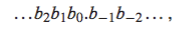
\includegraphics[width=3cm]{figs/general_form_of_binary_numbers.png} 
%%\caption{Mesh for the Finite Difference Method} 
%\end{figure}
而与这个二进制数相等的十进制数是
\begin{equation}
\ldots b_2 2^2 + b_1 2^1 + b_0 2^0 + b_{-1} 2^{-1} + b_{-2} 2^{-2} \ldots.
\end{equation}
例如
\begin{align}
(10101.1011)_2 = &1\cdot 2^4 + 0\cdot 2^3 + 1 \cdot 2^2 + 0 \cdot 2^1 + 1 \cdot 2^0  \nonumber \\
                             &+ 1\cdot 0.5 + 0\cdot0.25 + 1\cdot 0.125 + 1 \cdot 0.0625 \nonumber \\
                          = & 21.6875.
\end{align}

\end{frame}

\begin{frame}
\frametitle{二进制与十进制数}
我们用53.7为例介绍十进制数转换成二进制数的方法。首先,对于整数部分我们有
\begin{figure}
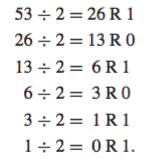
\includegraphics[width=2.5cm]{figs/decimal_to_binary_1.png} 
%\caption{Mesh for the Finite Difference Method} 
\end{figure}

\end{frame}

\begin{frame}
\frametitle{二进制与十进制数}
之后,对于小数部分我们有
\begin{figure}
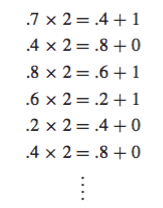
\includegraphics[width=3cm]{figs/decimal_to_binary_2.png} 
%\caption{Mesh for the Finite Difference Method} 
\end{figure}
因此,我们有$(53.7)_{10} = (110101.1\overline{0110})_2$. 我们可以看到一个重要现象:一个简单的十进制数往往是不能表示成为一个有限位的二进制数的。

\end{frame}


\subsection{浮点数}

\begin{frame}
\frametitle{IEEE浮点数}
计算机最为常用的储存数字的方式是浮点数。一个浮点数由三个部分组成:正负号、指数和尾数。例如,$9$这个数的二进制表示为$1001$,而浮点数表示为
\begin{equation}
0 \ 10 \ 001 
\label{floating point number general form}
\end{equation}
第一个部分的$0$表示该数是正数,第三个部分的尾数$001$表示的是这个数字的有效数字是$(1.001)_2$(默认起始位是$1$,因此这些数字叫作尾数),第二个部分的$(10)_2 = 3$表示的是这个数的指数为$3$,即得到这个数应该把小数点从有效数字处向右移动$3$位。这非常类似于科学计数法。例如53.7的科学计数法为
\begin{equation}
53.7 = + 5.37 *\times 10^1,
\end{equation}
而$(1001)_2$的\emph{归一化}表示为
\begin{equation}
(1001)_2 = + 1.001 \times 2^3.
\end{equation}


\end{frame}


\begin{frame}
\frametitle{双精度浮点数}
所谓双精度浮点数是指形如\eqref{floating point number general form}中的浮点数且其第二部分有$11$位,而第三部分有$52$位。例如$(9.4)_{10} = (1001.\overline{0110})_2$在双精度浮点数中的归一化表示为
\begin{figure}
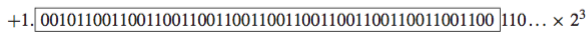
\includegraphics[width=8cm]{figs/double_precision_9-4.png} 
%\caption{Mesh for the Finite Difference Method} 
\end{figure}
其中方框中为尾数,而指数为$3$。我们再次看到,由于计算机可以储存的数字位数是有限的,$9.4$这样一个简单的数在计算机中并不是精确表示的,52位之后的数字会按照一定的规则进行舍入,因此会产生舍入误差。舍入的具体规则见参考教材[NA]的0.3章。

\end{frame}

\begin{frame}
\frametitle{绝对误差与相对误差}
我们利用浮点数的表示引入一些重要的定义和概念。
\begin{definition}[机器最小数]
机器$\epsilon$,用$\epsilon_{\mach}$表示,是指$1$与浮点数表示中比$1$大的第一个数之间的差。在IEEE双精度浮点数表示中,
\begin{equation}
\epsilon_{\mach} = 2^{-52}.
\end{equation}
\end{definition}

\begin{definition}[相对误差与绝对误差]
设$x_c$为精确值$x$的计算值,则
\begin{equation}
\text{绝对误差} = |x_c - x|,
\end{equation}
而
\begin{equation}
\text{相对误差} = \frac{|x_c - x|}{|x|}.
\end{equation}

\end{definition}

\end{frame}

\begin{frame}
\frametitle{浮点数的舍入误差}
我们有以下定理。
\begin{theorem}
假设${\rm{fl}}(x)$是$x$在{\rm{IEEE}}浮点数的表示规则中的机器表示,则
\begin{equation}
\frac{|{\rm{fl}}(x) - x|}{|x|} \le \frac{1}{2} \epsilon_{\mach}.
\end{equation}
\end{theorem}
可以看到,IEEE浮点数可以很好的控制数值的相对误差,但随着需要表示的数增大,绝对误差一般会相应变大,这是因为尾数的位数是一定的。\\
\ \\
\end{frame}

\subsection{浮点数的加法运算}

\begin{frame}
\frametitle{浮点数的加法运算}
浮点数的加法采用的是对位原则,即将两个加数的指数变为相同,之后将尾数相加,再将得数四舍五入之后储存为一个新的浮点数。我们用一个简单的例子$1+2^{-53}$来展示这个过程
\begin{figure}
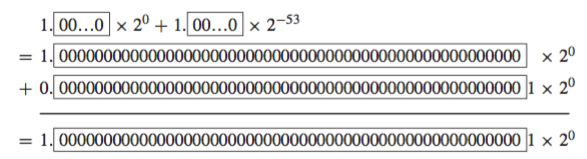
\includegraphics[width=9cm]{figs/floating_number_addition.png} 
%\caption{Mesh for the Finite Difference Method} 
\end{figure}
从上面所述的计算机加法我们注意到一点,$\epsilon_{\mach} = 2^{-52}$并不是具有双精度的计算机能够表示出的最小的数,但如果两数相加其中一个加数为$1$的话,那么$\epsilon_{\mach}$是另一个加数能够不被计算机忽略的最小值。

\end{frame}

\begin{frame}
\frametitle{计算机运算的不精确性}
由于计算机表示的精度有限和计算机加法的对位原则,计算机在运算时总会产生舍入误差。我们利用Matlab计算$9.4-9-0.4$来展示这种误差。


\end{frame}


\subsection{计算方法初步}
\begin{frame}
\frametitle{计算方法的重要性}
上面的例子显示计算机只能达到有限精度,因此每一次的计算都往往会产生误差,即误差是不可避免的。虽然如此,但是误差是可以通过计算方法的设计减小的。我们下面通过第一个例子说明,对于同一问题的计算,我们可以通过更好的计算方法使计算误差减少。我们通过第二个例子说明,对于同一问题,我们可以通过更好计算方法使得我们的计算速度提高。事实上,计算方法的两大重要性正是
\begin{enumerate}
\item 提高计算精度
\item 提高计算速度
\end{enumerate}

\end{frame}


\begin{frame}
\frametitle{利用算法避免有效数字丢失}
\begin{example}
假设我们有一台三位十进制计算机,利用它计算$\sqrt{9.01}-3$。
\end{example}

\begin{solution}
如果我们直接进行计算,由于$\sqrt{9.01} \approx 3.0016662$且我们使用的是三位的计算机,所以我们得到的在计算机中的结果应为$3.00$,因而最终的计算结果为$3.00-3 = 0$,很显然是一个错误的结果。如果我们将这个计算作一个等价变换,可以得到
\begin{figure}
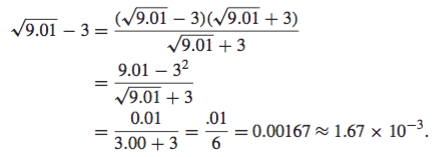
\includegraphics[width=6cm]{figs/loss_of_significant_numbers.png} 
%\caption{Mesh for the Finite Difference Method} 
\end{figure}
可以看到利用好的计算方法可以避免有效数字的丢失,提高计算精度。
\end{solution}

\end{frame}

\begin{frame}
\frametitle{利用算法提高多项式求值速度}
下面我们介绍著名的\emph{秦九韶}算法。假设我们有多项式
\begin{equation}
f(x) = a_0 + a_1 x + a_2 x^2 + \ldots + a_n x^n,
\label{eq:polynomial}
\end{equation}
如果直接进行多项式求值,则要求$f(x_0)$需要用$n + (n-1) + \ldots + 1 = \frac{n(n+1)}{2}$次乘法。现在将$f(x)$写为等价形式
\begin{equation}
f(x) = a_0 + x (a_1 + x(a_2 +x ( a_3 +\ldots x(a_{n-1}+ a_n x) \ldots),
\label{eq:polynomial_qinjiushao_equiv}
\end{equation}
(可以验证\eqref{eq:polynomial}和\eqref{eq:polynomial_qinjiushao_equiv}是等价的),则计算$f(x_0)$的值只需要用$n$次乘法。当$n$非常大的时候(例如1000),可以节省非常多的计算量(例如500倍左右)。

\end{frame}

\begin{frame}
\frametitle{利用算法提高多项式求值速度}
减少计算量除了有提高计算速度的作用之外,还可以间接提高计算精度。
\begin{example}
设$p(x) = (x-2)^9$。计算$f(x)$在区间$[1.92,2.08]$上的值。
\end{example}
\begin{solution}
如果将$p(x)$展开,我们有
\begin{align}
p(x) = (x-2)^9 = &x^9 - 18x^8 + 144x^7 - 672x^6 \nonumber \\
                          & 2016x^5 - 4032x^4 + 5376x^3 - 4608x^2 + 2304x -512.
\end{align}
我们将第一个等式的计算、第二个等式直接计算和第二个等式利用秦九韶算法计算的结果用以下三幅图展示出来。
\end{solution}

\end{frame}

\begin{frame}
\frametitle{利用算法提高多项式求值速度}
\begin{figure}
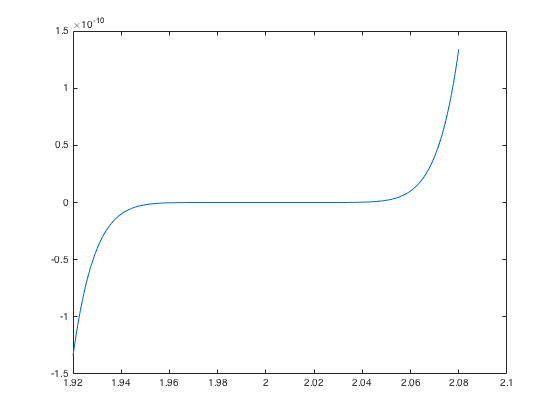
\includegraphics[width=7.5cm]{figs/f_simple.png} 
\caption{直接计算 $(x-2)^9$} 
\end{figure}

\end{frame}

\begin{frame}
\frametitle{利用算法提高多项式求值速度}
\begin{figure}
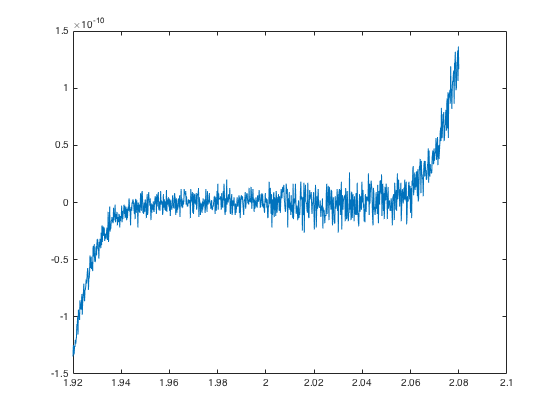
\includegraphics[width=7.5cm]{figs/f_direct.png} 
\caption{直接计算展开式} 
\end{figure}

\end{frame}

\begin{frame}
\frametitle{利用算法提高多项式求值速度}
\begin{figure}
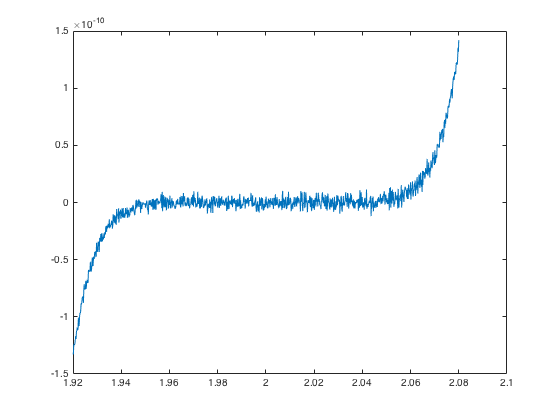
\includegraphics[width=7.5cm]{figs/f_nest.png} 
\caption{利用秦九韶算法计算展开式 } 
\end{figure}

\end{frame}

\begin{frame}
\frametitle{算法优劣的判定标准}
可以看到,减少计算的次数可以减少每一次计算所产生的舍入误差,进而间接提高计算精度。我们可以给一个比较一般的算法优劣的判定标准:
\begin{itemize}
\item 从截断误差观点看, 算法应当要截断误差小,收敛速度快,即运算量小,机器用时少。
\item 从舍入误差观点看,舍入误差在计算过程中要能控制,即算法要数值上稳定。
\item 从实现算法的观点看,算法的逻辑结构不宜太复杂,便于程序编制和上机实现。
\end{itemize}

\end{frame}


%%%%%%%%%%%%%%%%%%%%%%%%%%%%%%%%%%%%%%%%%%

\section{微积分知识回顾}
\begin{frame}
\frametitle{微积分知识回顾}
\begin{theorem}[中值定理]
设$f$是$[a,b]$上的连续函数,则$f$可以取得$f(a)$和$f(b)$之间的任何数,即假设$y$为$f(a)$和$f(b)$之间的任何一个数,则存在$c \in [a,b]$,使得$f(c) = y$.
\end{theorem}

\begin{theorem}[连续极限]
设$f$在$x_0$的某个临域上是连续函数且$\lim_{n \rightarrow \infty} x_n = x_0$。 则以下等式成立
\begin{equation}
\lim_{n \rightarrow \infty} f(x_n) = f(\lim_{n \rightarrow \infty} x_n) = f(x_0).
\end{equation}


\end{theorem}

\end{frame}

\begin{frame}
\frametitle{微积分知识回顾}
\begin{theorem}[微分中值定理]
设$f$是$[a,b]$上的连续可微函数(即$f$的导数$f'$仍然是连续函数),则存在$c \in [a,b]$使得
\begin{equation}
f'(c) = \frac{f(b)- f(a)}{b-a}.
\end{equation}
\end{theorem}

\begin{theorem}[Rolle定理]
设$f$是$[a,b]$上的连续可微函数且$f(a) = f(b)$,则存在$c \in [a,b]$,使得$f'(c) = 0$.
\end{theorem}


\end{frame}

\begin{frame}
\frametitle{微积分知识回顾}
\begin{theorem}[带余项的Taylor定理]
设$x$和$x_0$两个实数且$f$在$x$和$x_0$之间是$k+1$阶连续可导(即$f$的$1$到$k+1$阶导数均是连续的)。则存在$x$到$x_0$之间的数$c$使得
\begin{align}
f(x) = &f(x_0) + f'(x_0)(x-x_0) + \frac{f''(x_0)}{2!}(x-x_0)^2 + \frac{f''(x_0)}{3!}(x-x_0)^3  \nonumber \\
         &+ \ldots +\frac{f^{(k)}(x_0)}{k!}(x-x_0)^k +\frac{f^{(k+1)}(c)}{(k+1)!}(x-x_0)^{k+1}.
\end{align}
\end{theorem}

\begin{theorem}[积分中值定理]
设$f$是$[a,b]$上的连续函数,$g$是$[a,b]$上的可积函数且$g$在$[a,b]$上不变号。则存在$c \in [a,b]$,使得
\begin{equation}
\int_a^b f(x) g(x) \dx = f(c) \int_a^b g(x) \dx.
\end{equation}
\end{theorem}


\end{frame}


\begin{frame}
\frametitle{课后阅读}
[NA] 第0章


\end{frame}

\end{document}

